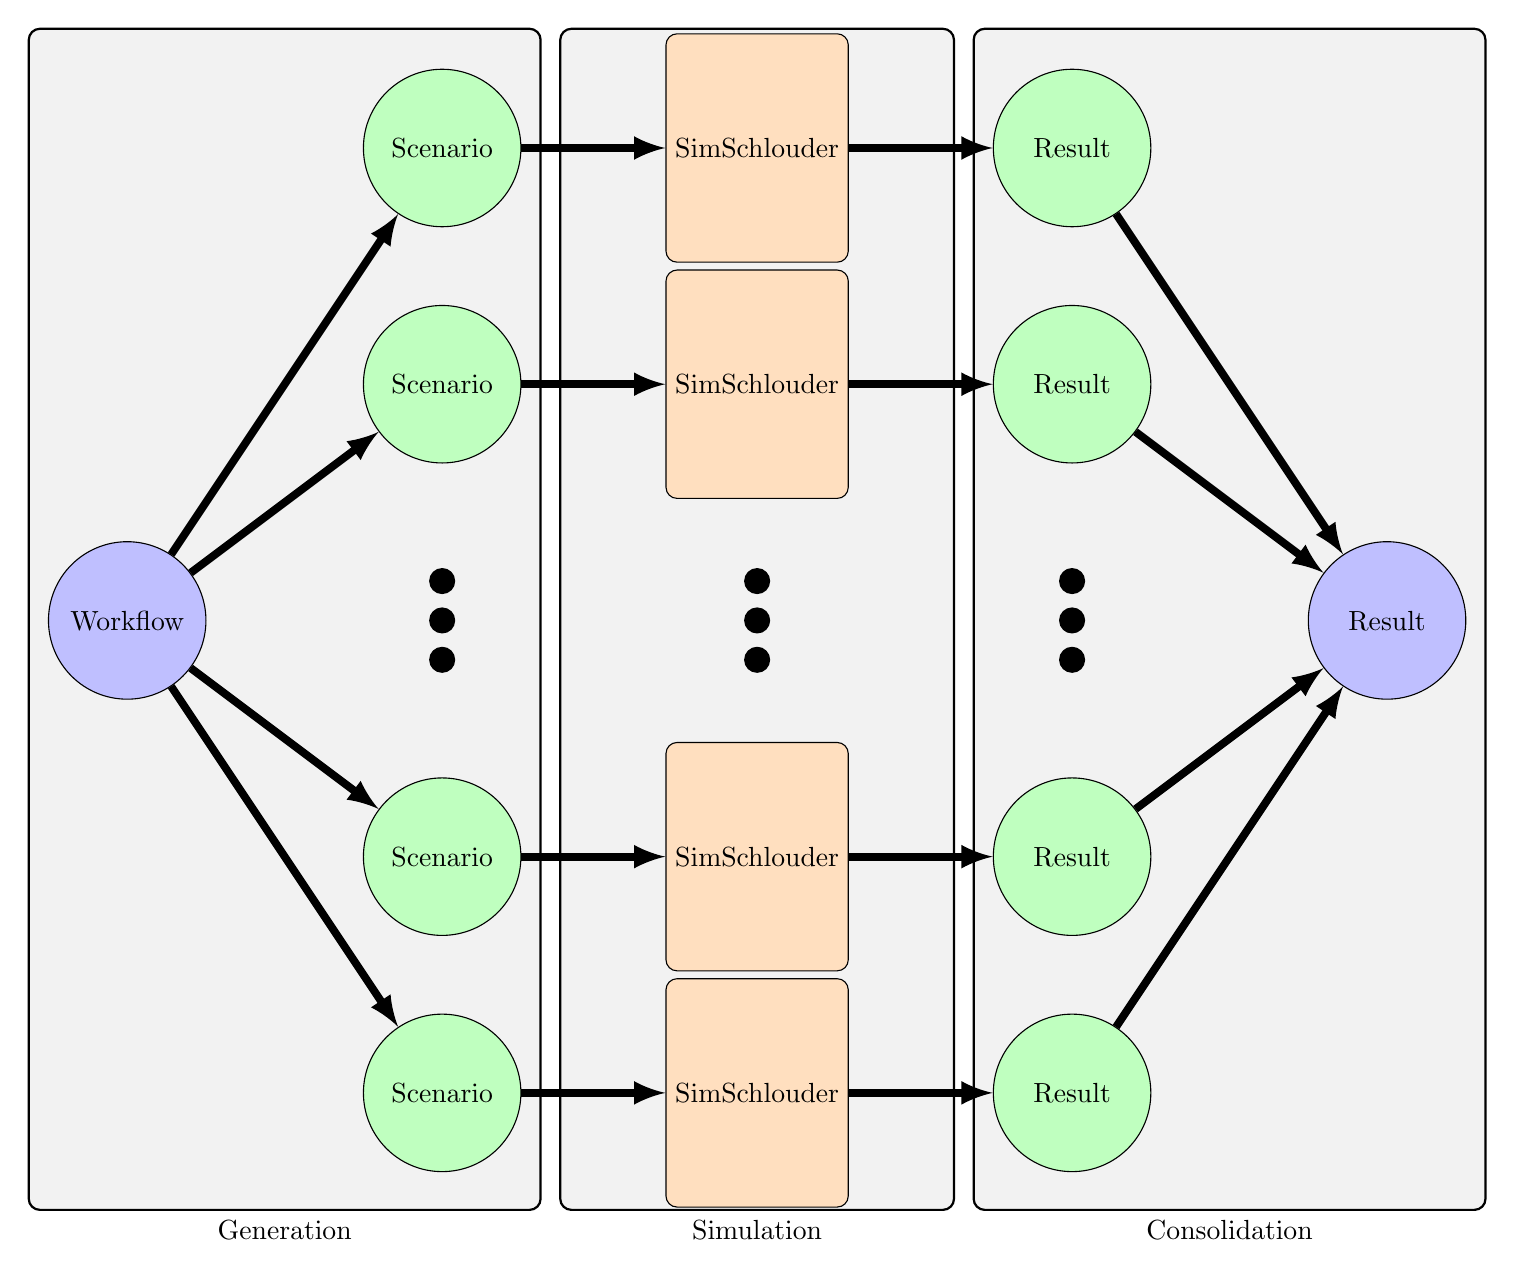
\begin{tikzpicture}[
x=5mm,
y=5mm,
sto/.style={%
draw,
circle,
minimum width=20mm,
fill=blue!25,
},
det/.style={%
draw,
circle,
minimum width=20mm,
fill=green!25,
},
dot/.style={%
circle,
fill=black,
minimum width=2mm
},
grp/.style={%
anchor=south,
minimum height=150mm,
draw,
thick,
rounded corners,
minimum width=25mm,
fill=black!5,
},
sim/.style={%
draw, 
rounded corners,
minimum height=29mm,
minimum width=23mm,
fill=orange!25,
}
]
%% Generation
\node[grp, minimum width=65mm, label={south:Generation}]at(4,-15){};
\node[sto]at(0,0)(init){Workflow};
\foreach \y in{1,2,-1,-2}{%
\node[det]at(8,6*\y)(g_\y){Scenario};
\draw[arrows=-latex,line width=1mm](init)--(g_\y);
}
%% Simulations
\node[grp, minimum width=50mm, label={south:Simulation}]at(16,-15){};
\foreach \y in{1,2,-1,-2}{%
\node[sim]at(16,6*\y)(s_\y){SimSchlouder};
\draw[arrows=-latex,line width=1mm](g_\y)--(s_\y);
}
%%Results
\node[grp, minimum width=65mm, label={south:Consolidation}]at(28,-15){};
\node[sto]at(32,0)(fin){Result};
\foreach \y in{1,2,-1,-2}{%
\node[det]at(24,6*\y)(r_\y){Result};
\draw[arrows=-latex,line width=1mm](s_\y)--(r_\y);
\draw[arrows=-latex,line width=1mm](r_\y)--(fin);
}
%% Black dots
\foreach \x in {8,16,24}{%
\foreach \y in {-1,0,1}{%
\node[dot]at(\x,\y){};
}
}
\end{tikzpicture}